\subsection{Surface Reconstruction}
\label{ssec:reconstruction}
In \autoref{sec:surfaceBackg} different surface reconstruction schemes were introduced. Here, we discuss our choice for an appropriate surface reconstruction scheme and explain necessary modifications to it.

\subsubsection{Discussion on Surface Reconstruction Schemes}
Since the surface reconstruction is just an intermediate step before our final \ac{NURBS} fitting procedure, it is not sufficient to only produce a good surface approximation of our optimized topology, but additional constraints have to be kept in mind:
\begin{itemize}
\item \ac{NURBS} have a rectangular topology, therefore our surface reconstruction should also be able to provide a surface consisting of rectangular patches.
\item Peters' Scheme only covers manifold surfaces. This means that each edge must be shared by exactly two patches.
\end{itemize}
The first requirement is met by \ac{DC}, while the second one is met only by \ac{MC}. Nevertheless, we decided to use the \ac{DC} method because its basic version already creates \acp{quad}, while \ac{MC} creates a mesh of triangles. This mesh can only be changed into a mesh of \acp{quad} by considerably increasing the number of faces.

\subsubsection{Our Implementation of Dual Contouring}
We use the open-source language PYTHON \cite{Python} for the implementation of \ac{DC}. Compared to the version described in \cite{Hermite2002} the following simplifications were applied:
\begin{itemize}
\item We use the simple averaging scheme described in \autoref{ssec:DC} instead of \autoref{eq:QEF}, since we do not consider sharp features and cannot easily access gradient information in our algorithm. 
\item Since our dataset only consists of boolean values instead of real valued quantities, we locate our surface at the material/non-material interface instead of a certain isovalue.
\item Our implementation does not support adaptivity or topology safety.
\end{itemize}
This leads to the following modified \ac{DC} scheme:
\begin{enumerate}
\item Find all sign-changing edges that connect material and non-material voxels.
\item On each sign-changing edge, find the root (i.e. the interface of material and non-material voxels) using bisection. We assume our surface to lie exactly in the middle of material and non-material voxels.
\item Take the mean value of these root positions for determining the position of the newly introduced vertex.
\item Join the vertices associated with four cubes sharing a common sign-changing edge to form a \ac{quad}.
\end{enumerate}
Thus our procedure generates \ac{quad} surfaces for boolean datasets on uniform Cartesian grids. But unlike the original \ac{DC} algorithm we cannot guarantee that these are manifold surfaces (see \autoref{sssec:nonmfsurf}).

\subsubsection{Obtaining Manifold Surfaces}
Since we want to deduce a first estimate for the topology of the \ac{NURBS} surface output, non-manifold surfaces cannot be accepted\footnote{Surfaces consisting of smoothly connected \ac{NURBS} \acp{patch} are always manifold surfaces. Therefore we cannot start with a non-manifold surface and assume we will end up with a manifold surface.}. We therefore use a remeshing procedure for generating manifold surfaces out of non-manifold surfaces. Our procedure has the following steps:
\begin{enumerate}
\item Find all non-manifold edges by searching for edges that are connected to more than two \acp{quad}.
\item For every non-manifold edge found, make a copy. Link the quads to the two resulting edges to create a manifold surface. Now, exactly two \acp{quad} are connected to each edge.
\item The member vertices of the original edge and those of its copy are moved in opposite directions. This is done to separate the overlapping edges. 
\end{enumerate}
We illustrate the procedure of remeshing for a 2D example in \autoref{fig:manifoldResolution2D}. 
In 3D we do not have non-manifold vertices, but edges, which have to treated. Please note that for the 3D case additional patterns come up. In 3D not only the \acp{quad} which are connected to the whole non-manifold edge have to be considered, but also the \acp{quad} connected to only one vertex of the edge. This also implies the introduction of new \acp{quad} at other locations. For an overview over some of the possible patterns in 3D see \autoref{fig:manifoldPatterns3D}.
\begin{figure}[t]
\begin{center}
\begin{subfigure}{.5\linewidth}
\centering
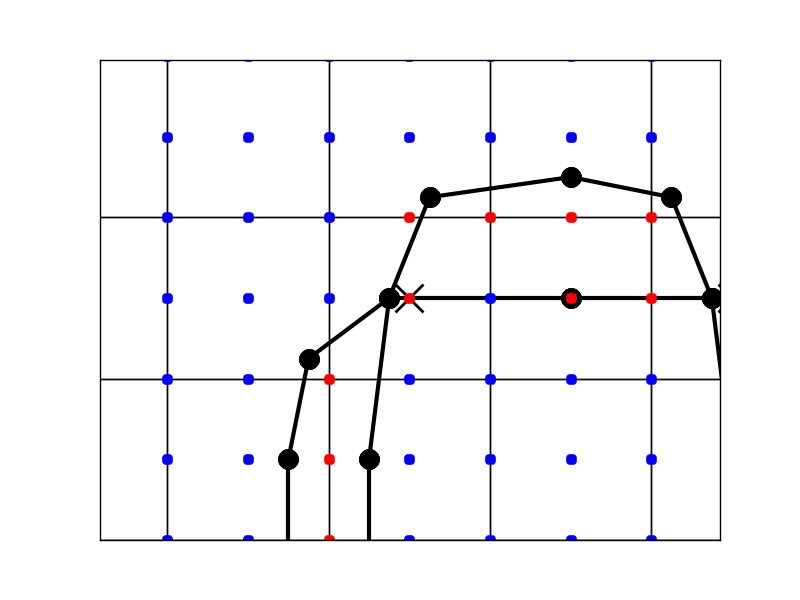
\includegraphics[width = \textwidth]{Pictures/SurfaceReconstruction/2DDoubleTorusNonManifoldDetail}
\subcaption{contour before remeshing}
\end{subfigure}%
\begin{subfigure}{.5\linewidth}
\centering
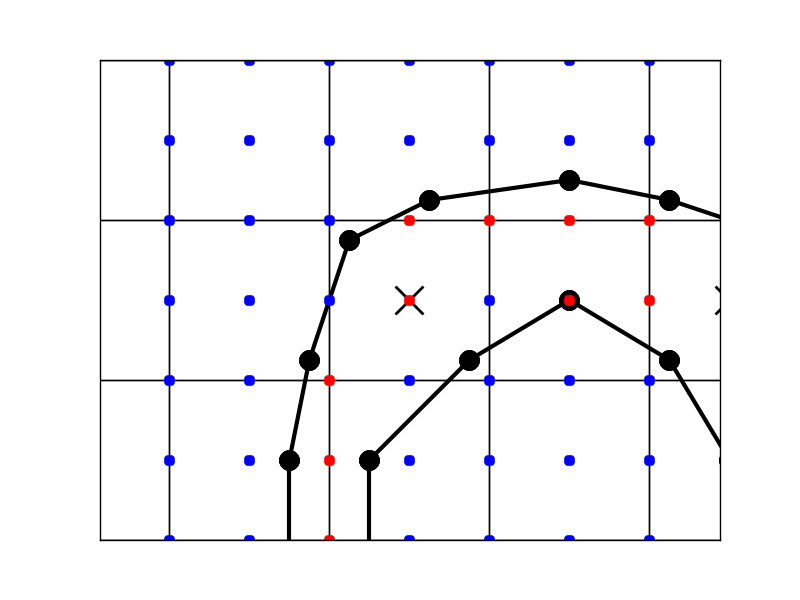
\includegraphics[width = \textwidth]{Pictures/SurfaceReconstruction/2DDoubleTorusManifoldDetail}
\subcaption{contour after remeshing}
\end{subfigure}
\end{center}
\caption{Illustration of the remeshing process. Blue dots denote outer voxels, red dots inner voxels. Crosses denote voxels considered for resolving ambiguities. We first copy the non-manifold vertex and then move the resulting pair of vertices in opposite directions. The direction is determined from the gradient at the datapoint with the cross, which goes in the direction of the blue dots (from inside to outside). Please note that we can only estimate the gradient if additional information is available in the middle of the cube which contains the non-manifold vertex. Otherwise it is not possible to resolve the ambiguity in a proper way and therefore we cannot eliminate the non-manifold vertex.}
\label{fig:manifoldResolution2D}
\end{figure}
\begin{figure}
\begin{center}
\begin{subfigure}[b]{.45\textwidth}
\centering
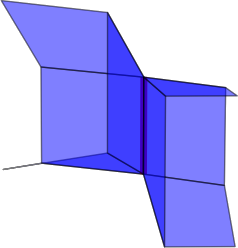
\includegraphics[height = .17\textheight, width = .5\textwidth,keepaspectratio]{Pictures/SurfaceReconstruction/3DManifoldOO}
\end{subfigure}
\begin{subfigure}[b]{.45\textwidth}
\centering
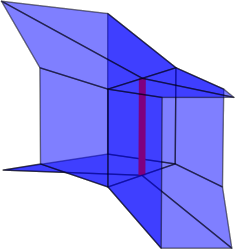
\includegraphics[height = .17\textheight, width = .5\textwidth,keepaspectratio]{Pictures/SurfaceReconstruction/3DManifoldOORes}
\end{subfigure}
\begin{subfigure}[b]{.45\textwidth}
\centering
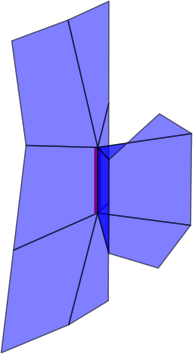
\includegraphics[height = .17\textheight, width = .5\textwidth,keepaspectratio]{Pictures/SurfaceReconstruction/3DManifoldII}
\end{subfigure}
\begin{subfigure}[b]{.45\textwidth}
\centering
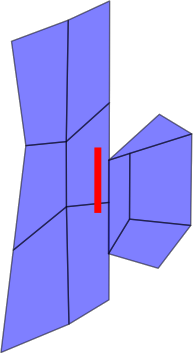
\includegraphics[height = .17\textheight, width = .5\textwidth,keepaspectratio]{Pictures/SurfaceReconstruction/3DManifoldIIRes}
\end{subfigure}
\begin{subfigure}[b]{.45\textwidth}
\centering
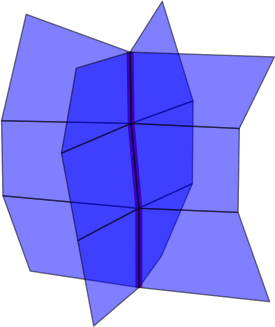
\includegraphics[height = .17\textheight, width = .5\textwidth,keepaspectratio]{Pictures/SurfaceReconstruction/3DManifoldMM}
\end{subfigure}
\begin{subfigure}[b]{.45\textwidth}
\centering
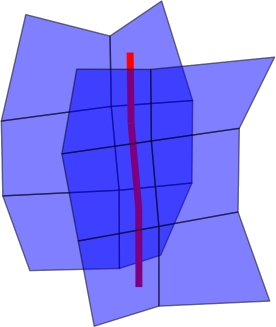
\includegraphics[height = .17\textheight, width = .5\textwidth,keepaspectratio]{Pictures/SurfaceReconstruction/3DManifoldMMRes}
\end{subfigure}
\begin{subfigure}[b]{.45\textwidth}
\centering
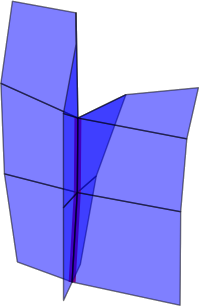
\includegraphics[height = .17\textheight, width = .5\textwidth,keepaspectratio]{Pictures/SurfaceReconstruction/3DManifoldMI}
\end{subfigure}
\begin{subfigure}[b]{.45\textwidth}
\centering
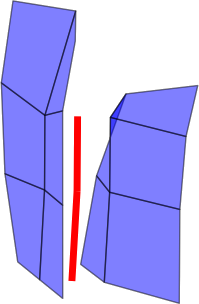
\includegraphics[height = .17\textheight, width = .5\textwidth,keepaspectratio]{Pictures/SurfaceReconstruction/3DManifoldMIRes}
\end{subfigure}
\begin{subfigure}[b]{.45\textwidth}
\centering
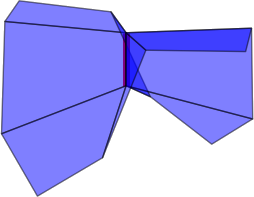
\includegraphics[height = .17\textheight, width = .5\textwidth,keepaspectratio]{Pictures/SurfaceReconstruction/3DManifoldOI}
\end{subfigure}
\begin{subfigure}[b]{.45\textwidth}
\centering
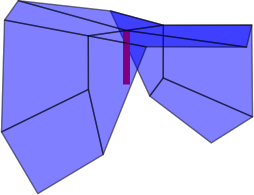
\includegraphics[height = .17\textheight, width = .5\textwidth,keepaspectratio]{Pictures/SurfaceReconstruction/3DManifoldOIRes}
\end{subfigure}
\end{center}
\caption{Different patterns before (left) and after (right) remeshing. Depending on the neighbourhood of the non-manifold edge (red) different patterns are applied. The edge is always copied. The resulting two edges are moved in opposite directions. A non-manifold edge is connected to outside-outside (1.row), inside-inside (2.row), two other manifold edges (3.row), inside and another manifold edge (4.row), inside-outside (5.row). In the first and last row copying the edge is not sufficient; new \acp{quad} have to be introduced. Please note that this figure does not cover all possible patterns.}
\label{fig:manifoldPatterns3D}
\end{figure}







\begin{comment}
\begin{table}
\begin{center}
\begin{tabularx}{.7\textwidth}{|*3{>{\centering\arraybackslash}X}|}
\hline
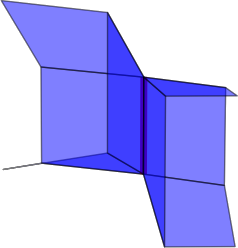
\includegraphics[height=.15\textheight]{Pictures/SurfaceReconstruction/3DManifoldOO}
&
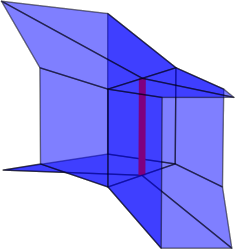
\includegraphics[height=.15\textheight]{Pictures/SurfaceReconstruction/3DManifoldOORes}
\\
\hline
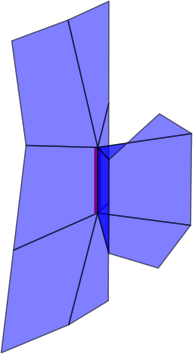
\includegraphics[height=.15\textheight]{Pictures/SurfaceReconstruction/3DManifoldII}
&
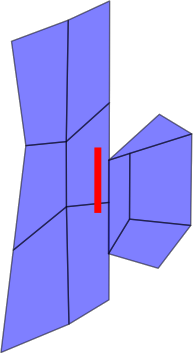
\includegraphics[height=.15\textheight]{Pictures/SurfaceReconstruction/3DManifoldIIRes}
\\
\hline
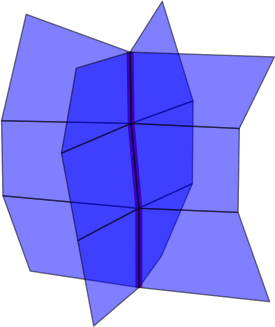
\includegraphics[height=.15\textheight]{Pictures/SurfaceReconstruction/3DManifoldMM}
&
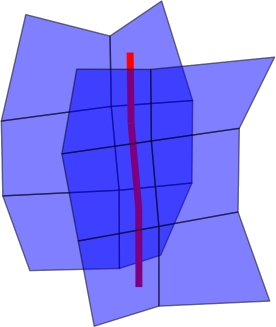
\includegraphics[height=.15\textheight]{Pictures/SurfaceReconstruction/3DManifoldMMRes}
\\
\hline
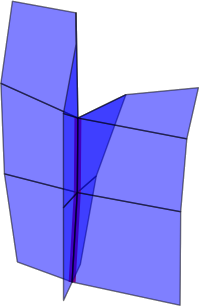
\includegraphics[height=.15\textheight]{Pictures/SurfaceReconstruction/3DManifoldMI}
&
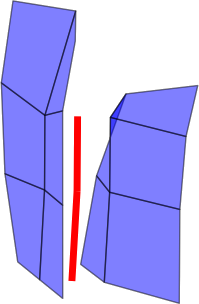
\includegraphics[height=.15\textheight]{Pictures/SurfaceReconstruction/3DManifoldMIRes}
\\
\hline
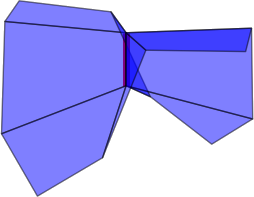
\includegraphics[height=.15\textheight]{Pictures/SurfaceReconstruction/3DManifoldOI}
&
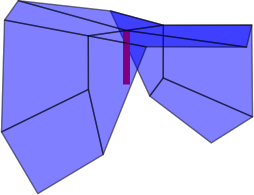
\includegraphics[height=.15\textheight]{Pictures/SurfaceReconstruction/3DManifoldOIRes}
\\
\hline
\end{tabularx}
\end{center}
\end{table}
\end{comment}

\begin{comment}
\begin{figure}[p]
\begin{minipage}[b][.17\textheight]{.45\textwidth}
\begin{center}
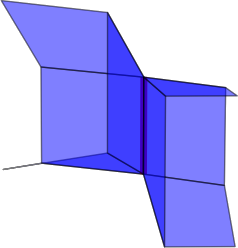
\includegraphics[height=.15\textheight]{Pictures/SurfaceReconstruction/3DManifoldOO}
\end{center}
\end{minipage}
\begin{minipage}[b][.17\textheight]{.45\textwidth}
\begin{center}
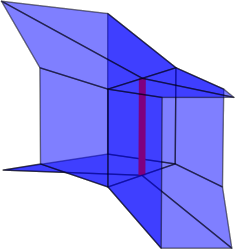
\includegraphics[height=.15\textheight]{Pictures/SurfaceReconstruction/3DManifoldOORes}
\end{center}
\end{minipage}
\begin{minipage}[b][.17\textheight]{.45\textwidth}
\begin{center}
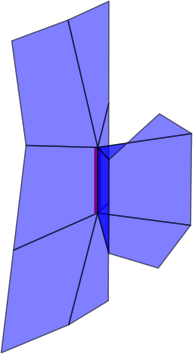
\includegraphics[height=.15\textheight]{Pictures/SurfaceReconstruction/3DManifoldII}
\end{center}
\end{minipage}
\begin{minipage}[b][.17\textheight]{.45\textwidth}
\begin{center}
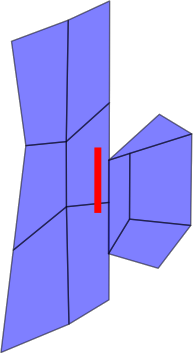
\includegraphics[height=.15\textheight]{Pictures/SurfaceReconstruction/3DManifoldIIRes}
\end{center}
\end{minipage}
\begin{minipage}[b][.17\textheight]{.45\textwidth}
\begin{center}
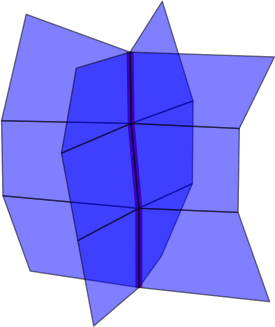
\includegraphics[height=.15\textheight]{Pictures/SurfaceReconstruction/3DManifoldMM}
\end{center}
\end{minipage}
\begin{minipage}[b][.17\textheight]{.45\textwidth}
\begin{center}
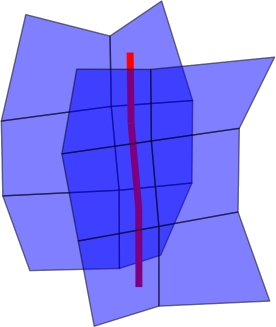
\includegraphics[height=.15\textheight]{Pictures/SurfaceReconstruction/3DManifoldMMRes}
\end{center}
\end{minipage}
\begin{minipage}[b][.17\textheight]{.45\textwidth}
\begin{center}
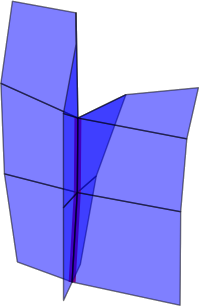
\includegraphics[height=.15\textheight]{Pictures/SurfaceReconstruction/3DManifoldMI}
\end{center}
\end{minipage}
\begin{minipage}[b][.17\textheight]{.45\textwidth}
\begin{center}
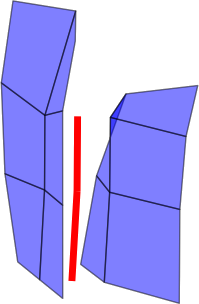
\includegraphics[height=.15\textheight]{Pictures/SurfaceReconstruction/3DManifoldMIRes}
\end{center}
\end{minipage}
\begin{minipage}[b][.17\textheight]{.45\textwidth}
\begin{center}
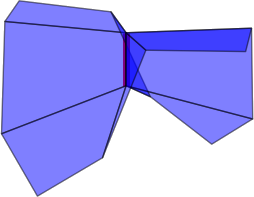
\includegraphics[height=.15\textheight]{Pictures/SurfaceReconstruction/3DManifoldOI}
\end{center}
\end{minipage}
\begin{minipage}[b][.17\textheight]{.45\textwidth}
\begin{center}
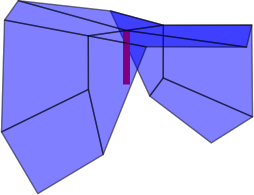
\includegraphics[height=.15\textheight]{Pictures/SurfaceReconstruction/3DManifoldOIRes}
\end{center}
\end{minipage}
\caption{Remeshing schemes for different kinds of manifold edges}
\label{fig:manifoldPatterns3D}
\end{figure}
\end{comment}

\begin{comment}

\subsubsection{Topology--safe adaptivity \ac{DC}}
\todo[inline]{Benni: this is a outlook, remove, put into comment.}
Implementing this feature in \ac{DC} will be one of our major goals in the future. Whether adding adaptivity to the basic \ac{DC} algorithm will destroy the property of \ac{DC} only generating \acp{quad} by introducing \acp{tri}, is going to be part of our future research.

\end{comment}
